\begin{figure}[t]
\centering
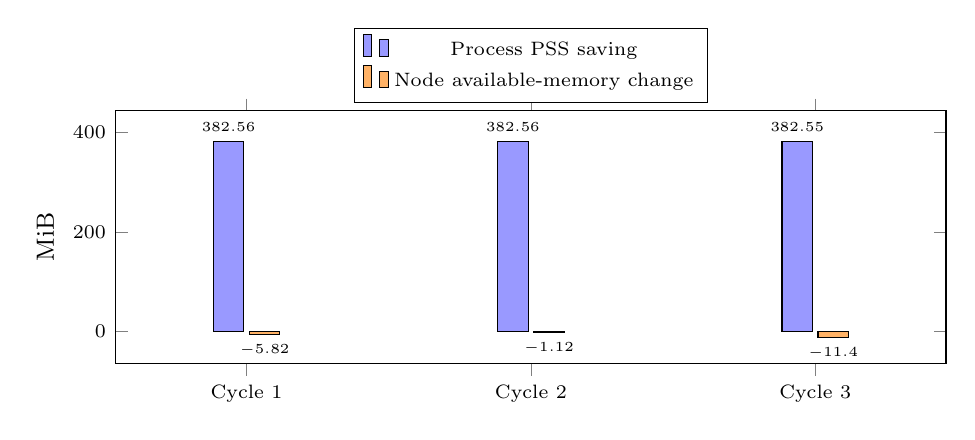
\begin{tikzpicture}
\begin{axis}[width=\columnwidth,height=4.8cm,ybar,bar width=11pt,ymin=-65,ymax=445,
 ylabel={MiB},symbolic x coords={Cycle 1,Cycle 2,Cycle 3},xtick=data,
 tick label style={font=\scriptsize},label style={font=\small},
 legend style={font=\scriptsize,at={(.5,1.03)},anchor=south,legend columns=1},
 nodes near coords,nodes near coords style={font=\tiny},enlarge x limits=.23]
\addplot[fill=blue!40] coordinates {(Cycle 1,382.56) (Cycle 2,382.56) (Cycle 3,382.55)};
\addplot[fill=orange!60] coordinates {(Cycle 1,-5.82) (Cycle 2,-1.12) (Cycle 3,-11.40)};
\legend{Process PSS saving,Node available-memory change}
\end{axis}
\end{tikzpicture}
\caption{Paired warmed Q4-to-Q3 observations. Positive PSS saving means a
smaller process footprint. Node availability does not increase in any cycle.
These metrics are not interchangeable or additive.}\label{fig:memory}
\end{figure}
